% THIS IS SIGPROC-SP.TEX - VERSION 3.1
% WORKS WITH V3.2SP OF ACM_PROC_ARTICLE-SP.CLS
% APRIL 2009
%
% It is an example file showing how to use the 'acm_proc_article-sp.cls' V3.2SP
% LaTeX2e document class file for Conference Proceedings submissions.
% ----------------------------------------------------------------------------------------------------------------
% This .tex file (and associated .cls V3.2SP) *DOES NOT* produce:
%       1) The Permission Statement
%       2) The Conference (location) Info information
%       3) The Copyright Line with ACM data
%       4) Page numbering
% 
\documentclass{acm_proc_article-sp}
\usepackage{comment}
\usepackage{url}
\usepackage{float}
\usepackage{needspace}

\begin{document}

\title{Modeling Temporal Evolution in the Endomondo Fitness Data Set}
%
\numberofauthors{2} % section.
%
\author{
\alignauthor
Yashodhan Hemant Karandikar\\
%       \email{ykarandi@ucsd.edu} \\
\bigskip
       {Advisor : Prof. Julian McAuley}
}


\maketitle
\begin{abstract}
The goal of this project is to model temporal evolution of runners' capacities across workouts as well as within each workout. We study this temporal evolution over 2 predictive tasks - prediction of duration and average-heart rate of the next workout given data of previous workouts and prediction of the next instantaneous heart-rate values in each workout. We evaluate these models on the Endomondo fitness data set \cite{endomondo} and provide some insight into the results.
\end{abstract}

% A category with the (minimum) three required fields
%\category{H.4}{Information Systems Applications}{Miscellaneous}
%A category including the fourth, optional field follows...
%\category{D.2.8}{Software Engineering}{Metrics}[complexity measures, performance measures]

%\terms{Theory}

%\keywords{Temporal evolution, fitness data sets, user modeling, heart-rate prediction} % NOT required for Proceedings

\section{Introduction}
People work out with the goal of becoming fitter. Regularly working out enables a person to take on more challenging work outs. For example, a runner training for long distance running can gradually attempt runs of longer durations. Thus, the running capacity or the fitness level of a runner increases gradually with practice. Modeling this fitness level can be useful in predicting the duration of the next workout that the runner attempts.

Alternatively, runners often monitor their heart-rate while running and set goals of keeping the heart-rate below or above a certain value, either for improving their fitness level or for their safety. The heart-rate at future instants in the run depends on how tired the runner currently is, among other factors. Further, this relationship between the heart-rate and how tired the runner is, varies from one runner to another. For example, an experienced runner might experience only a slight increase in heart-rate as he or she feels more tired, while the heart-rate of an amateur runner might shoot up soon after the run starts.

The examples above highlight the temporal evolution of a runner's capacity, both across workouts and within each workout. We attempt to model both these forms of temporal evolution in this work. Modeling such temporal evolution has several potential applications. Predictions of how long the next run will take, or the average and maximum heart-rates, will be useful both as a goal and as a guide to the runner while planning the run. Similarly, predicting how the heart-rate will change in the remaining part of a run will be useful for a runner who is monitoring heart-rate during the run. This can potentially be extended to suggest the runner a route for a run, given some desired parameters such as desired average heart-rate, desired total duration etc.

The rest of the report is organized as follows. Section \ref{secPredictiveTasks} describes the predictive tasks we will use to evaluate our models. Section \ref{secRelatedWork} describes some of the work in the literature which is relevant to temporal evolution of individuals and to these tasks. Section \ref{secDataset} describes the Endomondo data set \cite{endomondo}. Sections \ref{secBaselineModel}, \ref{secTemporalModelUsers} and \ref{secTemporalModelWorkouts} describe our models and the training and inference algorithms. Section \ref{secImplementationDetails} provides some implementation details of verifying correctness and achieving reasonable performance with our implementation. Section \ref{secEvaluation} discusses results of our models on the predictive tasks described in section \ref{secPredictiveTasks}. 

\section{Predictive Tasks}
\label{secPredictiveTasks}
In order to study temporal evolution of a runner \emph{across} several workouts, we choose the following 2 predictive tasks as follows:
\begin{enumerate}
\item Given the distance $d_i$ and duration $T_i$ for each workout $i$ for the first $n$ workouts of a runner $u$ and given the distance $d_{n+1}$ for the $(n+1)$'th workout, predict the duration $T_{n+1}$ of the $(n+1)$'th workout.
\item Given the distance $d_i$ and average heart-rate $H_i$ for each workout $i$ for the first $n$ workouts of a runner $u$ and given the distance $d_{n+1}$ for the $(n+1)$'th workout, predict the average heart-rate $H_{n+1}$ of the $(n+1)$'th workout.
\end{enumerate}

In order to study temporal evolution of a runner \emph{within} \emph{each} workout, we choose the following 2 predictive tasks as follows:

\begin{enumerate}
\item Given the first $n$ instantaneous heart-rate values of a runner in a workout, predict the $(n+1)$'th instantaneous heart-rate.
\item Given the instantaneous heart-rate values of the first $f$ fraction of a workout, predict the heart-rates of the remaining $1-f$ fraction of the workout. This task is a generalization of the first.
\end{enumerate}

\section{Related Work}
\label{secRelatedWork}
\cite{www13} describes 4 different models accounting for temporal evolution of user expertise through online reviews on websites such as Amazon, BeerAdvocate, RateBeer, CellarTracker. \cite{www13} describes these models along 2 orthogonal directions: individual/community evolution and evolution at uniform / learned intervals, for a total of 4 models. Of these, the model for individual evolution at learned intervals is the most general. Runners improve their physical capacities for working out at very different rates and independently of other runners, unlike general evolving trends in entire communities of users. Hence, the model for individual evolution at learned intervals makes most sense in the context of temporal evolution of runners' physical capacities for working out. The work in this project is based on this model.

Time-series analysis and prediction, studied extensively in literature \cite{timeSeriesStudy, timeSeriesSurvey, autoRegressiveModelWiki} are relevant to the task of predicting the instantaneous heart-rate values in the remaining workout.

\section{Endomondo Fitness data set}
\label{secDataset}
In this section, we introduce the Endomondo fitness data set \cite{endomondo}. Endomondo \cite{endomondo} is a free app and website that allows users to keep track of their workouts. The data extracted from the Endomondo website \cite{endomondo} is available in the form of a SQL dump of size 200 GB approximately after compression. It contains data for around 10 million workouts. Data for each workout is in the form of a HTML document string. This HTML document contains information about the workout such as the sport (such as running, walking, cycling etc.), user id, total distance, duration, wind, weather, hydration, date \& time etc. The HTML document also contains embedded JSON data. This JSON data contains GPS co-ordinates (latitude, longitude and altitude), distance, duration, heart-rate, speed / pace sampled throughout the duration of the workout. The `duration' trace indicates the time instants at which the remaining attributes were sampled. We developed a parser in Python to extract the relevant data from each HTML document, details of which are discussed in section \ref{secImplementationDetails}.

\subsection{Data set statistics}

We list some basic statistics of the data set. Table \ref{tableStatsTotal} lists the total number of workouts, the total number of users in the data set and the average number of workouts per user.

\begin{table}[h]
\centering
\begin{tabular}{|c|c|} \hline
Total number of workouts & 10320194  \\ \hline
Total number of users  &  2083006 \\ \hline
Avg. number of workouts per user & 4.95 \\ \hline
\end{tabular}
\caption{Number of workouts and users in the data set}
\label{tableStatsTotal}
\end{table}

Although the average number of workouts per user is only 4.95, the distribution of workouts among users is skewed, so that there are many users with more than 10 workouts. Table \ref{tableStatsUsers} lists number of users with more than 10, 40, 70, 100 workouts.

\begin{table}[h]
\centering
\begin{tabular}{|c|c|} \hline
\bf{$n$} & \bf{Number of users with more than $n$ workouts}  \\ \hline
10  &  271004        \\ \hline
40  &  11679   \\ \hline
70  &  2191  \\ \hline
100 &  768 \\ \hline
\end{tabular}
\caption{Number of users having more than 10, 40, 70, 100 workouts}
\label{tableStatsUsers}
\end{table}

Table \ref{tableStatsByActivity} lists the number of workouts for some of the activities (such as running, walking, cycling etc). The number of workouts for running is the highest and it is significantly more than that for other activities. Hence, in this work we use data from workouts for running only.

\begin{table}[h]
\centering
\begin{tabular}{|c|c|} \hline
\bf{Activity} & \bf{Number of Workouts}  \\ \hline
Running  &           4413262 \\ \hline
Walking  &           2154563 \\ \hline
Cycling, sport  &     938108 \\ \hline
Cycling, transport & 816808 \\ \hline
Mountain biking  &   429906 \\ \hline
Step counter     &   265403 \\ \hline
Fitness walking   &  172440 \\ \hline
Hiking &   147061 \\ \hline
\end{tabular}
\caption{Number of workouts by activity}
\label{tableStatsByActivity}
\end{table}


\section{Baseline Model}
\label{secBaselineModel}
This section describes a baseline model to predict the duration of a workout given the distance. Given the total distance $d_{ui}$ for the $i$'th workout of runner $u$, the predicted duration $T_{ui}'$ of the workout is given by:

\begin{equation}
\label{eqnBaselineDuration}
T_{ui}' = (\alpha + \alpha_{u})(\theta_0 + \theta_1 d_{ui})
\end{equation}

We have one parameter $\alpha_u$ per runner $u$, which is learned during training using runner $u$'s workouts. The parameters $\alpha, \theta_0, \theta_1$ are global to all runner. Thus, we have a total of $U + 3$ parameters, where $U$ is the number of distinct runners in the data set. 

Let $\Theta = (\alpha, \alpha_1, ... , \alpha_U, \theta_0, \theta_1)$. We need to find $\Theta$ which satisfies the following objective:

$$\hat{\Theta} = \arg\min_{\Theta}\frac{1}{|D|} \sum_{T_{ui} \in D}(T_{ui}' - T_{ui})^2 + \lambda \|\Theta \|_2^2 $$

where $D$ is the data set of all workouts for all runners, $T_{ui}$ is the true distance of workout $i$ of runner $u$. The term $\lambda \|\Theta \|_2^2$ is a regularizer. $\lambda$ is the regularization hyper-parameter, which we select by performing a line search over values in the set $\{0, 10^{-5}, 10^{-4},...,10^3, 10^{4}\}$ and choosing the $\lambda$ which minimizes the error on a validation set. We find the $\Theta$ which satisfies the objective using the L-BFGS \cite{lbfgs} implementation available in SciPy \cite{scipy}.

If the task is to predict the average heart-rate instead of the duration, we use the same model specification as equation \ref{eqnBaselineDuration} by replacing $T_{ui}'$ by $H_{ui}'$. Thus, the predicted average heart-rate is given by

$$H_{ui}' = (\alpha + \alpha_{u})(\theta_0 + \theta_1 d_{ui})$$


\section{Temporal Evolution Across \\ Workouts}
\label{secTemporalModelUsers}
This section generalizes the baseline model described in section \ref{secBaselineModel} and attempts to account for temporal evolution of runners across workouts. We describe the model, the training algorithm and finally the inference algorithm.

\subsection{Model Specification}
In order to account for evolution in the fitness level or capability of a runner over time,  we associate an \emph{experience level} or \emph{fitness level} $e_{uw}$ with each workout $w$ of runner $u$. This can be seen as a way of encoding how experienced the runner is at the time of the workout $w$. The value $e_{uw}$ is an integer in the interval $[0, E)$ where $E$ is the number of experience levels. 

Intuitively, we expect the experience level of a runner to either stay the same or increase with each workout. We encode this intuition in the form of a monotonicity constraint on the experience levels of workouts for each runner, as given below \cite{www13}:

$$\forall u,i,j \;\;\;\;\; t_{ui} \geq t_{uj} \implies e_{ui} \geq e_{uj}$$

where $t_{ui}$ is the time at which workout $i$ of runner $u$ occurs.

Then, given the total distance $d_{ui}$ for the $i$'th workout of runner $u$, the predicted duration $T_{ui}'$ of the workout is given by:

\begin{equation}
\label{eqnModelDuration}
T_{ui}' = (\alpha_{e_{ui}} + \alpha_{ue_{ui}})(\theta_0 + \theta_1 d_{ui})
\end{equation}


where $e_{ui}$ is the experience level of the runner $u$ at the $i$'th workout. Thus, we have one parameter $\alpha_{ue}$ per runner $u$ per experience level $e$. Further, we have an intercept term $\alpha_e$ for every experience level $e$, common to all runners. The terms $\theta_0$ and $\theta_1$ are global to all runners and experience levels. Thus, given $U$ runners and $E$ experience levels, we have a total of $UE + E + 2$ parameters.

Note that setting $E = 1$ reduces the model to the baseline model described in section \ref{secBaselineModel}.

We can specify a similar model for the predicted average heart rate $H_{ui}'$ of the runner $u$ during the workout $i$:

\begin{equation}
\label{eqnModelAvgHr}
H_{ui}' = (\alpha_{e_{ui}} + \alpha_{ue_{ui}})(\theta_0 + \theta_1 d_{ui})
\end{equation}

\subsection{Objective Function}
As explained above, we have a different model for each of the $E$ experience levels. Each of the $E$ models has the following parameters:

$$\Theta_e = (\alpha_e; \alpha_{1e}...\alpha_{Ue})$$

where $1 \leq e \leq E$ is the experience level and $U$ is the number of distinct runners.

Thus, all the parameters in all of the $E$ models together can be written as:

$$\Theta = (\Theta_1, \Theta_2,..., \Theta_E)$$

Let $\beta$ denote the set of all experience parameters $e_{ui}$. Then, we need to choose the optimal parameters $(\hat{\Theta}, \hat{\beta})$ according to the objective

%$$(\hat{\Theta}, \hat{\beta})  =  \arg\min_{\Theta,\beta}\frac{1}{|D|} \sum_{T_{ui} \in D}(T_{ui}' - T_{ui})^2 + \lambda_1\Omega_1(\Theta) + \lambda_2\Omega_2(\Theta, \theta_1) $$

\begin{align}
\label{eqnObjective}
(\hat{\Theta}, \hat{\beta})  &= \arg\min_{\Theta,\beta}\frac{1}{|D|} \sum_{T_{ui} \in D}(T_{ui}' - T_{ui})^2 \nonumber \\
 & + \lambda_1\Omega_1(\Theta) + \lambda_2\Omega_2(\Theta, \theta_1)
\end{align}

$$s.t. \; \; \; t_{ui} \geq t_{uj} \implies e_{ui} \geq e_{uj} $$

where $D$ is the data set of all workouts for all runners. This objective is similar to the one described in \cite{www13}. $\Omega_1$ and $\Omega_2$ are regularizers defined as follows:

$$\Omega_1(\Theta) = \sum_{e=1}^{E-1}{\|\Theta_e - \Theta_{e+1}\|_2^2}$$

and

$$\Omega_2(\Theta, \theta_1) = \theta_1^2 + \sum_{e=1}^{E}{\|\Theta_e \|_2^2}$$

$\Omega_1$ is a smoothness function which penalizes abrupt changes between successive experience levels \cite{www13}, since in practice similar experience levels should have similar parameters \cite{www13}. $\Omega_2$ is another regularizer which penalizes complex models i.e. it penalizes models which have higher magnitudes of parameters. These regularizers are necessary to avoid overfitting, since we have a large number $(UE + E + 2)$ of parameters. $\lambda_1$ and $\lambda_2$ are regularization hyperparameters, which trade-off the importance of regularization versus prediction accuracy at training time \cite{www13}. We select $\lambda_1$ and $\lambda_2$ through a grid-search over values in the set $\{0.0, 10^{-4}, 10^{-3},..., 10^4, 10^5\}$ and select the values which yield the highest prediction accuracy on a validation set.

For the task of predicting the average heart rate instead of the duration of the workout, the objective function remains the same as in equation \ref{eqnObjective}, except that the term $T_{ui}' - T_{ui}$ is replaced by $H_{ui}' - H_{ui}$.

\subsection{Training the model}
We optimize the parameters $\Theta$ and $\beta$ using a co-ordinate descent \cite{coordinateDescentWiki} i.e. we alternately optimize equation \ref{eqnObjective} for $\Theta$ given $\beta$ and $\beta$ given $\Theta$. We optimize the model parameters $\Theta$ given $\beta$ using L-BFGS \cite{lbfgs} available in the LibLBFGS library \cite{liblbfgs}. Optimizing $\beta$ given $\Theta$ means assigning a experience level to each workout so that the mean-squared-error is minimized, subject to the monotonicity constraint \cite{www13}. Since the experience levels are discrete, this problem is related to the \emph{Longest Common Subsequence} problem \cite{lcs} and can be solved efficiently using dynamic programming. The algorithm is identical to the one described in \cite{www13}.

We alternately optimize $\Theta$ given $\beta$ and $\beta$ given $\Theta$ until $\beta$ does not change or a maximum number of iterations has been reached.

\subsection{Inference}
Once the model parameters and experience levels have been learned, we infer i.e. predict the duration or average heart rate for the next workout $w$ using equation \ref{eqnModelDuration} or \ref{eqnModelAvgHr}. Note that we need to estimate the experience level for workout $w$ in order to be able to use equation \ref{eqnModelDuration} or \ref{eqnModelAvgHr} to predict the duration or average heart-rate. 

We perform inference in 2 modes, namely \emph{final} and \emph{random}, as is done in \cite{www13}. In the \emph{final} mode of inference, we use the first $N-2$ workouts as the training set, the $N-1$'th workout as the validation set and the $N$'th workout as the test set, where $N$ is the total number of workouts for a user $u$ in the data set. We assume $e_{u(N)} = e_{u(N-1)} = e_{u(N-2)}$ and use these experience levels to predict the duration (using equation \ref{eqnModelDuration}) or average heart rate (using equation \ref{eqnModelAvgHr}) for the examples in the validation and test set. The \emph{final} mode of inference is the setting that would be used in practice, since such a system would be used in predicting the duration or average heart-rate of the next workout instead of making predictions about past workouts \cite{www13}.

However, this mode of selecting workouts makes our validation and test sets biased towards workouts of more experienced runners \cite{www13}. To avoid this, we evaluate our models in the \emph{random} mode as well. In the \emph{random} mode of inference, we randomly select 1 workout as the validation set and 1 workout as the test set, for each runner. The experience levels for these workouts is assumed to be equal to those of the workouts closest in time in the training set for that runner. 

We present results for both modes of inference in section \ref{secEvaluation}.

\section{Temporal Evolution Within \\ Workouts}
\label{secTemporalModelWorkouts}
We now consider temporal evolution of a runner's capacity \emph{during} a workout and use it to predict the runner's instantaneous heart rate in the future. 

\subsection{Model Specification}

Given the heart-rate at various instants in a workout, we associate a \emph{tiredness level} $e_{wi}$ with heart-rate sample $i$ in the workout $w$. As before, the value $e_{wi}$ is an integer in the interval $[0, E)$, where $E$ is the number of tiredness levels. We expect the tiredness level of the user to either stay the same or increase with each sample in the workout. We encode this in the form of a monotonicity constraint as before:

$$\forall w,i,j \;\;\;\;\; t_{wi} \geq t_{wj} \implies e_{wi} \geq e_{wj}$$

where $t_{wi}$ is the time at which sample $i$ in workout $w$ was sampled.

Then, given the distance covered $d_{wt}$ at sample $t$ for the $w$'th workout, the predicted instantaneous heart-rate $h_{wt}'$ of the user is given by:

\begin{equation}
\label{eqnModelInstHr}
h_{wt}' = (\alpha_{e_{wt}} + \alpha_{we_{wt}})(\theta_0 + \theta_1 d_{wt})
\end{equation}

where $e_{wt}$ is the tiredness level at the $t$'th sample in workout $w$. Thus, as before, we have one parameter $\alpha_{we}$ per workout $w$ per tiredness level $e$ and an intercept term $\alpha_e$ for every tiredness level $e$, common to all workouts. The terms $\theta_0$ and $\theta_1$ are global to all workouts and tiredness levels. Thus, given $W$ workouts and $E$ tiredness levels, we have a total of $WE + E + 2$ parameters.

\subsection{Objective Function}
As before, we have a different model for each of the $E$ tiredness levels. Each of the $E$ models has the following parameters:

$$\Theta_e = (\alpha_e; \alpha_{1e}...\alpha_{We})$$

where $1 \leq e \leq E$ is the tiredness level and $W$ is the number of workouts in the data set.

Thus, all the parameters in all of the $E$ models together can be written as:

$$\Theta = (\Theta_1, \Theta_2,..., \Theta_E)$$

Let $\beta$ denote the set of all tiredness levels $e_{wt}$. Then, we need to choose the optimal parameters $(\hat{\Theta}, \hat{\beta})$ according to the objective

\begin{align}
\label{eqnObjective2}
(\hat{\Theta}, \hat{\beta})  &= \arg\min_{\Theta,\beta}\frac{1}{|D|} \sum_{h_{wt} \in D}(h_{wt}' - h_{wt})^2 \nonumber \\
 & + \lambda_1\Omega_1(\Theta) + \lambda_2\Omega_2(\Theta, \theta_1)
\end{align}

$$s.t. \; \; \; t_{wi} \geq t_{wj} \implies e_{wi} \geq e_{wj} $$

where $D$ is the data set of all samples in all workouts. This objective is similar to the one described in \cite{www13}.

As before, $\Omega_1$ and $\Omega_2$ are regularizers defined as follows:

$$\Omega_1(\Theta) = \sum_{e=1}^{E-1}{\|\Theta_e - \Theta_{e+1}\|_2^2}$$

$$\Omega_2(\Theta, \theta_1) = \theta_1^2 + \sum_{e=1}^{E}{\|\Theta_e \|_2^2}$$

$\Omega_1$ is a smoothness function which penalizes abrupt changes between successive tiredness levels \cite{www13}, since in practice similar tiredness levels should have similar parameters \cite{www13}. $\Omega_2$ is another regularizer which penalizes complex models i.e. it penalizes models which have higher magnitudes of parameters. These regularizers are necessary to avoid overfitting, since we have a large number $(WE + E + 2)$ of parameters. $\lambda_1$ and $\lambda_2$ are regularization hyperparameters, which trade-off the importance of regularization versus prediction accuracy at training time \cite{www13}. We select $\lambda_1$ and $\lambda_2$ through a grid-search over values in the set $\{0.0, 10^{-4}, 10^{-3}, 10^{-2}, 10^{-1}, 10^{0}\}$ and select the values which yield the highest prediction accuracy on a validation set.

\subsection{Training the model}
The training algorithm is identical to the training algorithm described in section \ref{secTemporalModelUsers}.

\subsection{Inference}
Once the model parameters and tiredness levels have been learned, we infer i.e. predict the instantaneous heart rate at 1 instant in each workout $w$ using equation \ref{eqnModelInstHr}. As before, we need to estimate the tiredness level at that instant in order to be able to use equation \ref{eqnModelInstHr} to predict the instantaneous heart-rate. 

As in section \ref{secTemporalModelUsers}, we perform inference in  2 modes, namely \emph{final} and \emph{random}.  In the \emph{final} mode of inference, we use the first $N-2$ samples in each workout as the training set, the $N-1$'th sample from each workout as the validation set and the $N$'th sample as the test set, where $N$ is the total number of samples in a workout. We assume $e_{wN} = e_{w(N-1)} = e_{w(N-2)}$ and use these tiredness levels to predict the instantaneous heart-rate using equation \ref{eqnModelInstHr}.

In the \emph{random} mode of inference, we randomly select 1 sample from each workout as the validation set and 1 sample from each workout as the test set. The tiredness levels for these samples is assumed to be equal to those of the samples closest in time in the training set. 

We present results for both modes of inference in section \ref{secEvaluation}.

\subsection{Prediction of several instantaneous heart rate values}
We now generalize the problem of predicting 1 instantaneous heart-rate value to the problem of predicting the heart-rate values for the last $f$ fraction of the workout. We use the same model as described earlier in this section. Let $e_{wn}$ be the tiredness level of the last sample in workout $w$ in the training set. In order to predict the instantaneous heart-rate values in the remaining part of the workout, we assume $e_{wn} = e_{w(n+1)} = e_{w(n+2)} = ... = e_{w(N)}$ where $N$ is the total number of samples in workout $w$. In other words, we assume that the last tiredness level of the workout fitted during training stays the same for the remaining part of the workout. In practice, this is not a valid assumption, but this provides us with a conservative estimate of how well the model performs on the remaining part of the workout i.e. on the validation and test sets.

Note that the difficulty here is not only that of estimating the tiredness levels accurately, but also not having learned model parameters for tiredness levels beyond the last tiredness level fitted during training. Thus, even if the true tiredness levels for the remaining part of the workout are known, these cannot be used for prediction of heart-rate values.

\section{Implementation Details}
\label{secImplementationDetails}

\subsection{Extracting relevant data}
As mentioned in section \ref{secDataset}, the data extracted from the Endomondo website \cite{endomondo} is available in the form of a SQL dump of size 200 GB approximately after compression. It contains data for around 10 million workouts. Data for each workout is in the form of a HTML document string. We developed a parser in Python to extract the relevant data from each HTML document.  We use parallelization to speed-up the extraction of the data. Each line of the SQL dump contains data for multiple workouts in the form of HTML documents. A `master' process reads each line, extracts the HTML documents and hands them over to `worker' processes. Each `worker' process takes 1 HTML document at a time, parses it to extract the relevant information about the workout and encodes it into a dictionary in JSON format. The worker then queues this workout data into a global queue. A separate `writer' process dequeues workout information and writes it to a single file in the form of 1 line per workout. Having a separate writer process to write the workouts extracted by worker processes eliminates disk contention among workers. It also allows data for all workouts to be written to a single large file instead of millions of small files, without any need for synchronization between processes since only a single process is performing the writes. All of the extracted data is written to a file of size around 30 GB after compression.

\subsection{Performance optimizations}

We use Python for most of the data processing tasks, with NumPy \cite{numpy} and SciPy \cite{scipy} libraries. We observe that the training is computationally the most intensive part of the execution. We first speed-up the training using Cython \cite{cythonNumpy}. This gives considerable speed-ups and scales well for the tasks of predicting duration and average heart-rate for the next workout of a user. However, even with this optimization, training still remained prohibitively expensive for the large data sets involved in the task of predicting instantaneous heart-rate values (see  section \ref{secEvaluation} for details of the data sets). Hence, we port the training part of these tasks to C++. This gives much higher speed-ups and enables the training process for a single run to complete in a few minutes on a personal laptop machine.

\subsection{Verifying Correctness}

We verify that our implementations of derivative functions are correct by comparing their outputs to those obtained by computing numerical derivatives. We use functions provided in \cite{scipy} and \cite{dlib} to compute numerical derivatives.

%\needspace{2\baselineskip}
\section{Evaluation}
\label{secEvaluation}
This section describes the results of the models described in sections \ref{secTemporalModelUsers} and \ref{secTemporalModelWorkouts} on the predictive tasks described in section \ref{secPredictiveTasks}. For all the tasks, we consider only workouts of the sport `running' in the dataset.

\subsection{Temporal evolution across workouts}
This section discusses results of the model described in section \ref{secTemporalModelUsers} on the tasks of predicting the average heart-rate and total duration of a runner's next workout.

\subsubsection{Prediction of average heart-rate}

For this task, we consider only workouts of runners having more than 10 workouts. Further, we discard workouts with invalid date/time (i.e. a timestamp of 0), extremely long workouts (greater than 100 mi), extremely short workouts (lesser than 0.1 mi), workouts with extremely high average heart-rate (greater than 500 bpm) and workouts with extremely low average heart-rate (lesser than 10 bpm). We also discard workouts which do not have either heart-rate information or distance information.

Tables \ref{tableAvgHrFinal} and \ref{tableAvgHrRandom} show results for prediction of average heart-rate, using the  \emph{final} and \emph{random} modes of evaluation, as discussed in \ref{secTemporalModelUsers}. As discussed in section \ref{secTemporalModelUsers}, we have 1 workout in the validation set and 1 workout in the test set for each runner in the data set, for both modes of evaluation. The results are shown in terms of the coefficient of determination, $R^2$ \cite{r2Wiki}, which is a measure of the fraction of variance in the data explained by the model. Table \ref{tableAvgHrHyperparams} shows the optimal values of hyper-parameters found using grid search.

As seen from the results, the model which accounts for temporal evolution of users does not perform better than the baseline model ($E = 1$). A closer look at the hyper-parameters resulting from the grid search, as shown in table \ref{tableAvgHrHyperparams}, gives us some insight into this result. As is seen from table \ref{tableAvgHrHyperparams}, grid search yields high optimal values of $\lambda_1$. Recall from section \ref{secTemporalModelUsers} that $\lambda_1$ is a hyper-parameter which penalizes drastic changes in parameters of similar experience levels. A high value of $\lambda_1$ means that the experience levels are very similar to each other and this essentially reduces the models with $E = 2$ and $E = 3$ to the baseline model $E = 1$.

\begin{table}[h]
\centering
\begin{tabular}{|c|c|c|c|} \hline
& Training $R^2$ & Validation $R^2$ & Test $R^2$ \\ \hline
\# Examples & 39545 & 2384 & 2384  \\ \hline
Baseline($E = 1$)& 0.520887 & 0.422324 & 0.423512 \\ \hline
$E = 2$ & 0.520928 & 0.422081 & 0.423318 \\ \hline
$E = 3$ & 0.520927 & 0.422085 & 0.423312 \\ \hline
\end{tabular}
\caption{Prediction of avg. heart-rate - \emph{Final} mode of evaluation }
\label{tableAvgHrFinal}
\end{table}

\begin{table}[h]
\centering
\begin{tabular}{|c|c|c|c|} \hline
& Training $R^2$ & Validation $R^2$ & Test $R^2$ \\ \hline
\# Examples & 39545 & 2384  &  2384 \\ \hline
Baseline ($E = 1$) & 0.517636 & 0.481049 & 0.430987 \\ \hline
$E = 2$  & 0.517645 & 0.480964 & 0.430880 \\ \hline
$E = 3$  & 0.517692 & 0.480968 & 0.430886 \\ \hline
\end{tabular}
\caption{Prediction of avg. heart-rate - \emph{Random} mode of evaluation }
\label{tableAvgHrRandom}
\end{table}

\begin{table}[h]
\centering
\begin{tabular}{|c|c|c|} \hline
& $\lambda_1$ & $\lambda_2$ \\ \hline
$E = 2$ (final) & $10^4$ & $0.0$ \\ \hline
$E = 3$ (final) & $10^5$ & $0.0$ \\ \hline
$E = 2$ (random) & $10^5$ & $0.0$ \\ \hline
$E = 3$ (random) & $10^4$ & $0.0$ \\ \hline
\end{tabular}
\caption{Optimal values of hyper-parameters $\lambda_1$ and $\lambda_2$ for prediction of average heart-rate}
\label{tableAvgHrHyperparams}
\end{table}

To get some insight into this result, we plot the average error for each workout number, averaged over all users, as shown in figure \ref{figAvgHrAvgErrorE1}. If the data set contains a significant evolution of the user's experience from the user's 1st workout to the last, we expect to see the average error higher for some workout numbers compared to others. However, figure \ref{figAvgHrAvgErrorE1} shows that the average error is roughly constant with respect to the workout number, indicating there is no significant evolution of user experience in the data set. This explains the lack of improvement in the $R^2$ score achieved with the models with $E = 2$ and $E = 3$.

\begin{figure}[h]
\centering
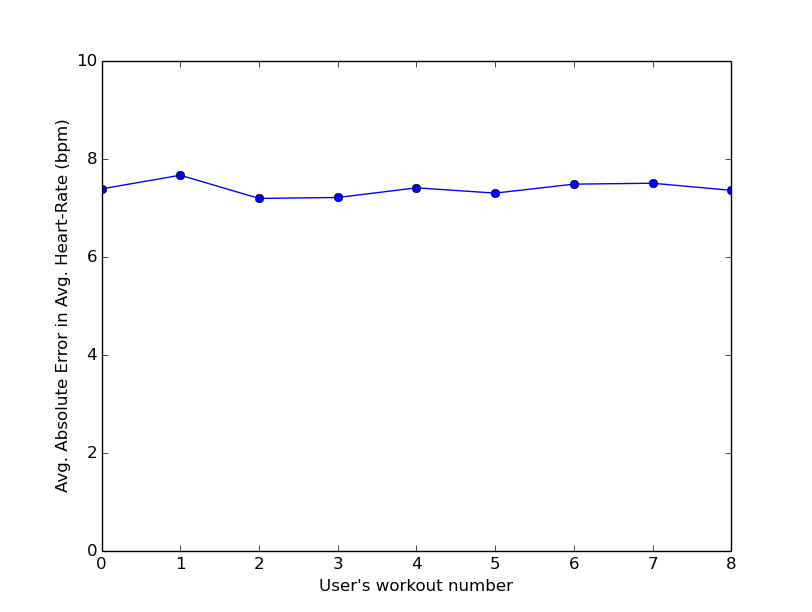
\includegraphics[scale=0.35]{../src/plots/avghr_error_vs_workout_E1}
\caption{\label{figAvgHrAvgErrorE1}  Average error in prediction of the average heart-rate for each workout number, averaged over all users, over the training set.}
\end{figure}

\subsubsection{Prediction of duration}

For this task, we consider only workouts of runners having more than 10 workouts. Further, we discard workouts with invalid date/time (i.e. a timestamp of 0), extremely long workouts (greater than 100 mi and/or 72 hours), extremely short workouts (lesser than 0.1 mi and/or 36 seconds). We also discard workouts which do not have either duration information or distance information.

Tables \ref{tableDurationFinal} and \ref{tableDurationRandom} show results for the prediction of the duration of the workout, using the  \emph{final} and \emph{random} modes of evaluation, as discussed in \ref{secTemporalModelUsers}. As discussed in section \ref{secTemporalModelUsers}, we have 1 workout in the validation set and 1 workout in the test set for each runner in the data set, for both modes of evaluation. The results are shown in terms of the coefficient of determination, $R^2$ \cite{r2Wiki}. Table \ref{tableDurationHyperparams} shows the optimal values of hyper-parameters found using grid search.

The model which accounts for temporal evolution of runners performs marginally better than the baseline model in the \emph{final} mode of evaluation, but this is not true in the \emph{random} mode of evaluation. Further, as is seen from table \ref{tableDurationHyperparams}, grid search yields relatively high optimal values of $\lambda_1$, indicating that the experience levels are very similar to each other and this essentially reduces the models with $E = 2$ and $E = 3$ to the baseline model $E = 1$.

\begin{table}[H]
\centering
\begin{tabular}{|c|c|c|c|} \hline
& Training $R^2$ & Validation $R^2$ & Test $R^2$ \\ \hline
\# Examples & 743987 & 52109 & 52109 \\ \hline
Baseline ($E = 1$) & 0.785361 & 0.677276 & 0.696565 \\ \hline
$E = 2$ & 0.775247 & 0.677833 & 0.714295 \\ \hline
$E = 3$ & 0.782736 & 0.677098 & 0.718808 \\ \hline
\end{tabular}
\caption{Prediction of duration - \emph{Final} mode of evaluation }
\label{tableDurationFinal}
\end{table}

\begin{table}[H]
\centering
\begin{tabular}{|c|c|c|c|} \hline
& Training $R^2$ & Validation $R^2$ & Test $R^2$ \\ \hline
\# Examples & 743987 & 52109 & 52109  \\ \hline
Baseline ($E = 1$) & 0.736994 & 0.627867 & 0.596432 \\ \hline
$E = 2$ & 0.691232 & 0.627357 & 0.578873 \\ \hline
$E = 3$ & 0.705088 & 0.634563 & 0.581045 \\ \hline
\end{tabular}
\caption{Prediction of duration - \emph{Random} mode of evaluation }
\label{tableDurationRandom}
\end{table}

\begin{table}[H]
\centering
\begin{tabular}{|c|c|c|} \hline
& $\lambda_1$ & $\lambda_2$ \\ \hline
$E = 2$ (final) & $10^4$ & $0.001$ \\ \hline
$E = 3$ (final) & $10^2$ & $0.001$ \\ \hline
$E = 2$ (random) & $10$ & $0.01$ \\ \hline
$E = 3$ (random) & $10$ & $0.01$ \\ \hline
\end{tabular}
\caption{Optimal values of hyper-parameters $\lambda_1$ and $\lambda_2$ for prediction of duration of the workout}
\label{tableDurationHyperparams}
\end{table}

As in the case of the prediction of average heart-rate, we plot the average error for each workout number, averaged over all users, as shown in figure \ref{figDurationAvgErrorE1}. We observe that the average error is roughly constant with respect to the workout number, indicating there is no significant evolution of user experience in the data set. This explains the lack of improvement in the $R^2$ score achieved with the models with $E = 2$ and $E = 3$.

\begin{figure}[h]
\centering
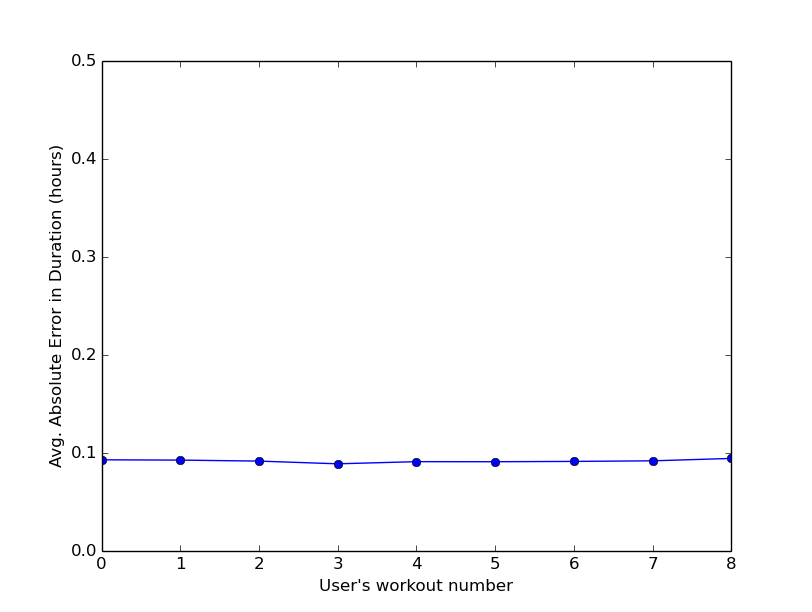
\includegraphics[scale=0.35]{../src/plots/duration_error_vs_workout_E1}
\caption{\label{figDurationAvgErrorE1}  Average error in prediction of the duration for each workout number, averaged over all users, over the training set.}
\end{figure}

The lack of improvement in the prediction accuracy after accounting for temporal evolution across workouts seem to suggest that we need data for many more workouts per runner and over much longer periods of time in order to be able to notice a reasonably strong evolution of the runner across workouts.

\subsection{Temporal evolution within workouts}

We now discuss results for temporal evolution \emph{within} workouts. First, we discuss results for the task of predicting a single instantaneous heart-rate value in each workout, followed by prediction of several instantaneous heart-rate values in each workout.

\subsubsection{Prediction of 1 heart-rate value}

For this task, we consider only workouts with at least 200 samples of instantaneous heart-rate values and distance values. Tables \ref{tableInstHrFinal} and \ref{tableInstHrRandom} show results for the task of predicting a single instantaneous heart-rate value in each workout, using the \emph{final} and \emph{random} modes of evaluation respectively. Accounting for temporal evolution within each workout significantly improves the prediction accuracy over the baseline ($E = 1$), for both modes of evaluation.

\begin{table}[H]
\centering
\begin{tabular}{|c|c|c|c|} \hline
& Training $R^2$ & Validation $R^2$ & Test $R^2$ \\ \hline
\# Examples & 24347765 & 83423  & 83423  \\ \hline
Baseline ($E = 1$) & 0.608874 & 0.585329 & 0.560480 \\ \hline
$E = 10$ & 0.887163 & 0.839256 & 0.799058 \\ \hline
$E = 20$ & 0.944594 & 0.899215 & 0.853857  \\ \hline
\end{tabular}
\caption{Prediction of instantaneous heart-rate - \emph{Final} mode of evaluation }
\label{tableInstHrFinal}
\end{table}

\begin{table}[H]
\centering
\begin{tabular}{|c|c|c|c|} \hline
& Training $R^2$ & Validation $R^2$ & Test $R^2$ \\ \hline
\# Examples & 24347765  & 83423  & 83423  \\ \hline
Baseline ($E = 1$) & 0.613856 & 0.608207 & 0.615789 \\ \hline
$E = 10$ & 0.907340 & 0.894736 & 0.897766 \\ \hline
$E = 20$ & 0.944524 & 0.928297 & 0.928000 \\ \hline
\end{tabular}
\caption{Prediction of instantaneous heart-rate - \emph{Random} mode of evaluation }
\label{tableInstHrRandom}
\end{table}

We plot the average absolute error in the prediction of instantaneous heart-rate against the sample number within the workout, averaged over all workouts in the training set. Figure \ref{figInstHrErrorVsSample} shows this plot for both $E = 20$ and the baseline $E = 1$. We observe that the plot for $E = 1$ shows non-uniform errors for various sample numbers, unlike the plots shown in figures \ref{figAvgHrAvgErrorE1} and \ref{figDurationAvgErrorE1}. This indicates that the data set contains temporal evolution of the heart-rate within every workout and thus explains the improvement in $R^2$ score achieved by the models with $E = 10$ and $E = 20$. Figure \ref{figInstHrErrorVsSample} shows the average errors for the model with $E = 20$ as well. We observe that the average errors for $E = 20$ are significantly lesser than those for the baseline model $(E = 1)$, as expected.

\begin{figure}[h]
\centering
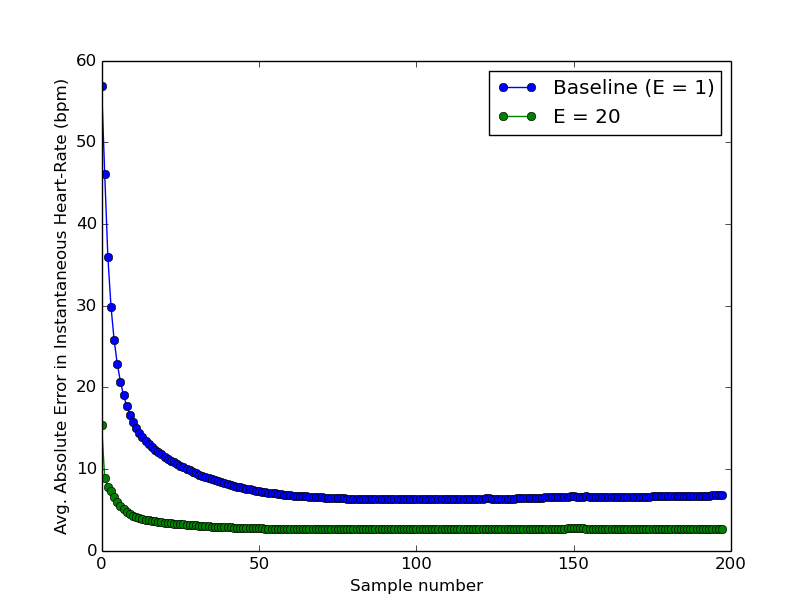
\includegraphics[scale=0.4]{../src/plots/insthr_error_vs_sample_comparison}
\caption{\label{figInstHrErrorVsSample} Average error in prediction of the instantaneous heart-rate for each sample number, averaged over all workouts in the training set.}
\end{figure}

Figure \ref{figR2vsTirednessLevels} shows how the prediction accuracy on the training and validation sets increases as we increase the number of tiredness levels $E$. 
%The optimal value of $E$ is $E = 20$, beyond which the prediction accuracy decreases. This plot is done using the \emph{final} mode of evaluation.

\begin{figure}[h]
\centering
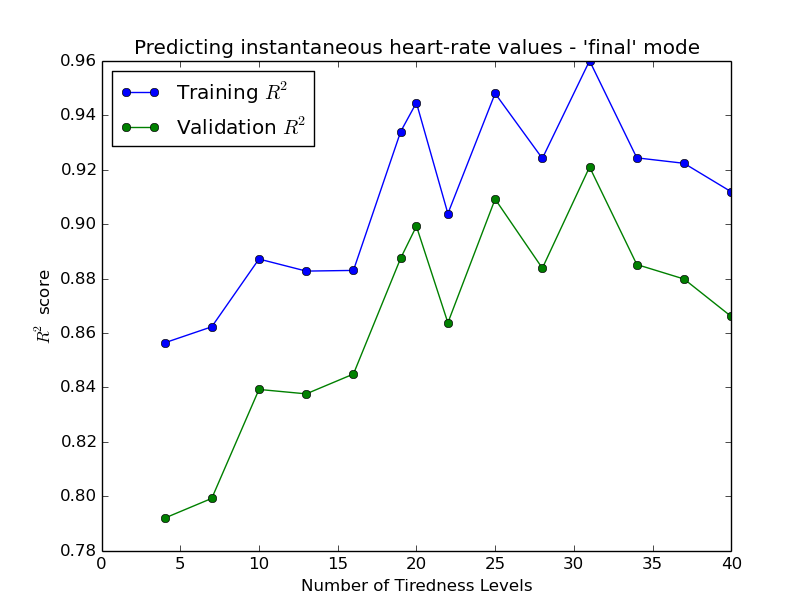
\includegraphics[scale=0.4]{../src/plots/r2_vs_num_tiredness_levels}
\caption{\label{figR2vsTirednessLevels} $R^2$ score on training and validation sets with varying number of tiredness levels.}
\end{figure}

\needspace{2\baselineskip}
\subsubsection{Prediction of last several heart-rate values}
Runners often monitor their heart-rate while running and set goals of keeping the heart-rate below or above a certain value. Accordingly, a prediction of next several instantaneous heart-rate values would be more useful for the runner instead of a prediction of just the next 1 heart-rate value. This is one of the potential applications of this work. Hence, in this section, we evaluate how well our model predicts the heart-rate values in the remaining part of the workout.

For this task, we consider only workouts with at least 200 samples of instantaneous heart-rate values and distance values. Given a workout of $N \geq 200$ samples of instantaneous heart-rate and distance values, we split $N$ (distance, heart-rate) samples into training, validation and test sets of sizes $0.4N$, $0.3N$, $0.3N$ respectively. Table \ref{tableInstManyHr} shows results for the task of predicting last several instantaneous heart-rate values in each workout. The results indicate that accounting for temporal evolution significantly improves results compared to the baseline. 

\begin{table}[H]
\centering
\begin{tabular}{|c|c|c|c|} \hline
& Training $R^2$ & Validation $R^2$ & Test $R^2$ \\ \hline
\# Examples &  9841317 & 7352229 & 7321065 \\ \hline
Baseline ($E = 1$) & 0.567424 & 0.451540 & 0.356603 \\ \hline
$E = 10$ & 0.911437 & 0.632749 & 0.464435 \\ \hline
$E = 20$ &  0.926065 & 0.633388 & 0.458077 \\ \hline
\end{tabular}
\caption{Prediction of several instantaneous heart-rates in each workout}
\label{tableInstManyHr}
\end{table}

We observe that the $R^2$ scores on the validation set are much higher than those for the test set. This is expected due to the fact that the samples in the test set are further in time than the samples in the validation set, which in turn are further in time than the samples in the training set. Recall from section \ref{secTemporalModelWorkouts} that we assume $e_{wn} = e_{w(n+1)} = e_{w(n+2)} = ... = e_{w(N)}$ where $N$ is the total number of samples in workout $w$ and $e_{wn}$ is the last sample in workout $w$ in the training set. This assumption is lesser likely to hold for samples further and further in time. Thus, this assumption is less likely to hold for the test set than for the validation set. Hence, the $R^2$ scores on the test set are lower than on the validation set, which in turn are lower than on the training set. This can be seen from the plot shown in figure \ref{figManyInstHrErrorVsSampleNumberValTest}. The $X$ axis is the sample number since the last sample in the training set. The $Y$ axis is the absolute error averaged over all workouts. As expected, the average absolute error increases as the sample is further in time.

\begin{figure}[h]
\centering
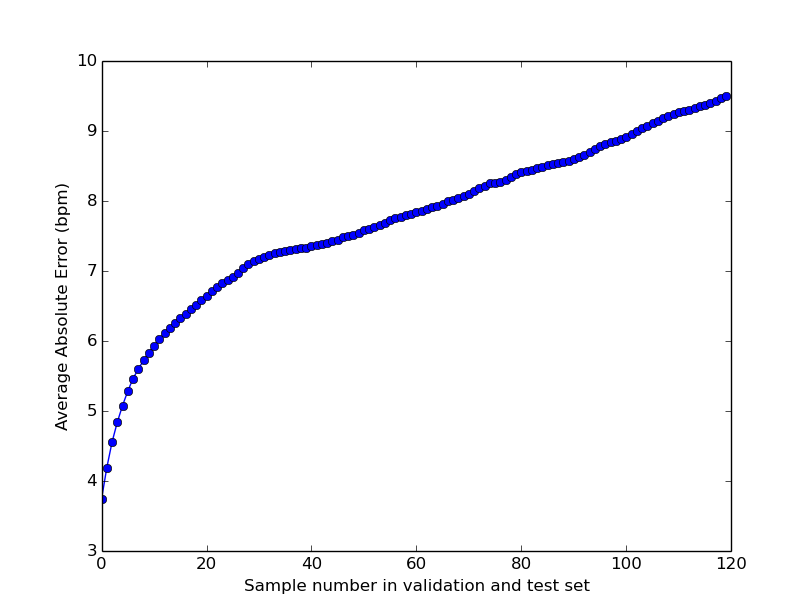
\includegraphics[scale=0.4]{../src/plots/many_insthr_error_vs_sample_number}
\caption{\label{figManyInstHrErrorVsSampleNumberValTest} Average absolute error versus the sample number in the workout after the training samples, averaged over all workouts in the validation and test set, for $E = 20$}
\end{figure}

\section{Conclusion and Future Work}
We describe and evaluate 2 different ways of accounting for temporal evolution of runners' physical capacities for running workouts - one \emph{across} workouts and the other \emph{within} workouts. Results indicate that accounting for temporal evolution across workouts does not improve prediction accuracy, perhaps due to the relatively small number of workouts per runner in the data set. On the other hand, accounting for temporal evolution \emph{within} each workout significantly improves results over the baseline model.

Future work includes evaluating these models for other types of workouts, such as cycling, walking etc. The results on these types of workouts might give some interesting insights about the nature of these activities and about how users evolve with time in each of these activities. It might be interesting to repeat this work for a much larger data set with many workouts per user, since temporal evolution across workouts might be more prominent in such a data set. Models for time series prediction such as auto-regression \cite{autoRegressiveModelWiki} can also be used to predict the instantaneous heart-rate in the remaining workout.


\bibliographystyle{abbrv}
\bibliography{references.bib}

\end{document}
